\documentclass{scrartcl}
\usepackage[latin1]{inputenc}
\usepackage[T1]{fontenc}
\usepackage[ngerman]{babel}
\usepackage{amsmath}
\usepackage{amssymb}
\usepackage{icomma}
%\usepackage[dvips]{graphicx}
%\usepackage{floatflt}
%\usepackage{enumitem}
%\usepackage{babel}
\usepackage{blindtext}
%\usepackage{showframe}
\usepackage{calc}
\usepackage{wrapfig}
\def\BILD{\rule{0.4\textwidth}{4cm}}

\usepackage{graphicx}
\usepackage{placeins}
\usepackage{multirow}
\usepackage{subfig}
\usepackage{url}

\renewcommand{\topfraction}{.85}
\renewcommand{\bottomfraction}{.7}
\renewcommand{\textfraction}{.15}
\renewcommand{\floatpagefraction}{.66}
\renewcommand{\dbltopfraction}{.66}
\renewcommand{\dblfloatpagefraction}{.66}
\setcounter{topnumber}{9}
\setcounter{bottomnumber}{9}
\setcounter{totalnumber}{20}
\setcounter{dbltopnumber}{9}
\setlength{\intextsep}{0cm plus1cm minus1cm}
\pdfminorversion = 5
\usepackage{setspace}
\onehalfspacing

\begin{document}
\title{Versuch 5: Millikan-Versuch}


\date{01.11.2010}


\author{Gruppe 5a: Gia-Danh Lam, Nils Haldenwang}

\maketitle
\tableofcontents

\section{Einleitung}
Elektrische Ladungen treten nur in gequantelten Werten als Vielfache
$n \cdot e$ der Elementarladung $e$ auf mit $ n \in \mathbb{Z}$. Im
Jahr 1910 gelang es Robert Andrews Millikan die Elementarladung $e$
relativ genau zu bestimmen, er erhielt $ e = 1.592 \cdot 10^{-19}C$
und daf�r sp�ter auch einen Nobelpreis. Nach heutigem Kenntnisstand
betr�gt der Wert $ e = 1,602 176 487 (40) \cdot 10^{-19} C$. Millikan
ist nicht der alleinige Erfinder des nach ihm benannten Versuches, er
griff auf vorherige Arbeiten von Harold Albert Wilson und Joseph John
Thomson zur�ck und verbesserte diese ma�geblich.

Zum Messen der Elementarladung werden �ltr�pfchen in einen
Kondensator, dessen Feld parallel zum Gravitationsfeld der Erde
ausgerichtet ist gebracht. Die untersuchten Tr�pfchen tragen nur einige wenige
Elementarladungen. Legt man keine Spannung an den Kondensator an, so
fallen die Tropfen mit einer konstanten Geschwindigkeit nach unten. Da
sie also offenbar nicht mehr beschleunigt werden, muss ein
Gleichgewicht der wirkenden Kr�fte vorliegen. Die wirkenden Kr�fte
sind in diesem Fall die Schwerkraft $F_g$, die Auftriebskraft $F_a$ und die
Reibungskraft $F_R$.

Schaltet man nun den Kondensator ein, so kommt die elektrostatische
Kraft $F_e$ des elektrischen Feldes auf das Tr�pfchen hinzu. Die
Richtung von $F_e$ ist je nach Polung unterschiedlich und ist somit
leicht umkehrbar. Nat�rlich �ndert sich mit der Bewegungsrichtung des
Tr�pfchens auch die Richtung der Reibungskraft $F_R$.

Der Aufbau und die Kr�fte sind schematisch in Abb. \ref{fig: Kraefte}
dargestellt.

\begin{figure}%[htb!]
\centering
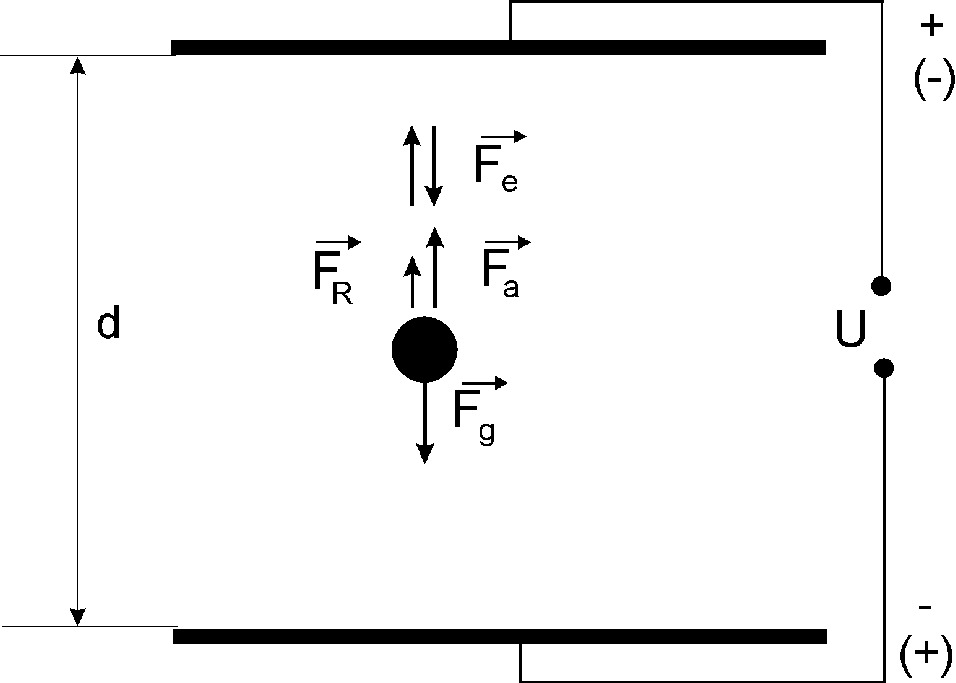
\includegraphics[width=12cm]{pics/SchemaAufbau}%
\caption{Schematischer Aufbau des Versuchs mit den wirkenden Kr�ften.}%
\label{fig: Kraefte}%
\end{figure}

\section{Dimensionsanalyse}
Wir wollen hier nur kurz �berpr�fen, ob bei der Gleichung 11
% nochmal gucken
auch die Einheiten beider Seiten �bereinstimmen. Auf der linken Seite
erkennt man sofort, dass die Einheit Coulomb ist. Auf der rechten
Seite gelingt es uns nicht mit einem Blick auf die Einheit Coulomb zu
schlie�en. Daher analysieren wir diesen Term:
\begin{equation}
q=\frac{4\pi g\rho_{\text{�}l}}{3}\left(\sqrt{\left(\frac{b}{2p}\right)^{2}+\frac{9\eta v_{\downarrow}}{2\rho_{\text{�}l}g}}-\frac{b}{2p}\right)^{3}\frac{\left(v_{\downarrow}+v_{\uparrow}\right)}{v_{\downarrow}}\frac{d}{U}
\label{eq:1}
\end{equation}
\[\left[\frac{4\pi g\rho_{\text{�}l}}{3}\right]\left(\sqrt{\left[\left(\frac{b}{2p}\right)^{2}\right]+\left[\frac{9\eta v_{\downarrow}}{2\rho_{\text{�}l}g}\right]}-\left[\frac{b}{2p}\right]\right)^{3}\left[\frac{\left(v_{\downarrow}+v_{\uparrow}\right)}{v_{\downarrow}}\right]\left[\frac{d}{U}\right]\]
\[=\frac{kg m}{s^2 m^3} \left(\sqrt{\frac{Pa^2m^2}{Pa^2}+\frac{kg m^4 s^2}{kg m^2 s^2}}+\frac{Pam}{Pa}\right)^3 \frac{m}{s}\frac{s}{m} \frac{m}{V}=\frac{kgm}{s^2m^3}m^3\frac{As^3m}{kg m^2}=As=C\]
Die Einheiten stimmen ,wie erwartet, �berein.

\section{Einrichten der Messanordnung}
Der Versuch geschieht auf einer Messplattform, die in der H�her und Ausrichtung ver�ndert werden kann. Auf dieser befinden sich eine Lampe, die die Messkammer ausleuchtet, eine Libelle, um die Messplattform m�glichst horizontal einzustellen, Anschl�sse f�r den Thermisator, welcher die Temperatur in der Messkammer misst und die Messkammer mit einem eingebautem Mikroskop zur Beobachtung der in der Messkammer zu findenden �ltr�pfchen. An ihr ist ein Drehhebel angebracht, den man auf die Stellung "`on"' ,"`off"' und auf den "`spray droplet position"' drehen kann. Hierbei wird bei "`off"' der Raum zwischen den beiden Kondensatoren vollkommen geschlossen, bei der "`spray droplet position"' wird das Loch des Plastikstiftes "`droplet hole cover"' ge�ffnet und bei "`on"' wird die Messkammer durch ein Thoriumpr�parat mit $\alpha$-Strahlung bestrahlt. Beobachtet wird der Versuch  auf einem Bildschirm, welcher mit einer Kamera verbunden ist, die auf das Mikroskop gerichtet ist. Der Aufbau ist in Abb. \ref{fig:Messplattform} zu sehen. Der genaue Aufbau der Messkammer ist in Abb. \ref{fig:Messkammer} dargestellt.
\vspace{\baselineskip}

\begin{figure}[hbp!]
\begin{minipage}{9cm}
	\centering
	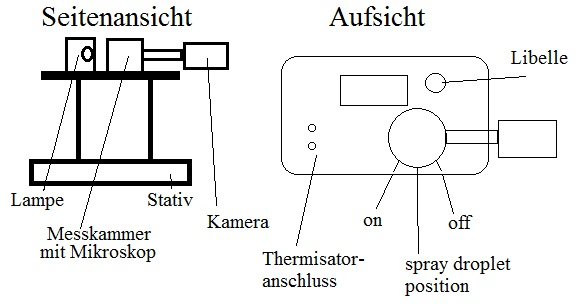
\includegraphics[width=9cm]{pics/Messplattform}
	\caption{Seiten- und Aufsicht der Messplattform}
	\label{fig:Messplattform}
\end{minipage}
\hfill
\begin{minipage}{6cm}
	\centering
	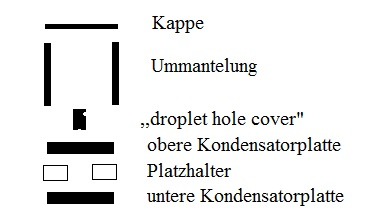
\includegraphics[width=6cm]{pics/Messkammer}
	\caption{Aufbau der Messkammer}
	\label{fig:Messkammer}
\end{minipage}
\end{figure}
\vspace{\baselineskip} Um ein gutes Bild auf dem Bildschirm sehen zu
k�nnen muss sowohl das Mikroskop als auch die Kamera eingestellt
werden. Zun�chst wird das Okular des Mikroskops so verschoben, dass
das Bild des Gitter, welches sich in der Zwischenbildebene befindet,
scharf wird. Das Objektiv muss auch verschoben werden. Hierzu wird
kurz ein Draht durch das Loch in der oberen Kondensatorplatte in die
Messkammer gehalten und dann wird durch Verstellen des Objektivs das
Bild des Drahtes scharf gestellt. Nun wird noch die Kameraeinstellung
so ver�ndert, dass das Bild des Gitters stark vergr��ert und relativ
klar auf dem Bildschirm zu sehen ist. Dies dient zur Messung der
Geschwindigkeiten der �ltr�pfchen, da der Abstand von zwei dicken
waagerechten Linien auf dem Bildschirm genau 0.5mm betr�gt. Das Bild
wird damit um mehr als 10.000 mal vergr��ert. Zuletzt werden durch
einen Zerst�uber �ltr�pfchen zwischen die Kondensatorplatte gespr�ht.
Mit einem

\end{document}

